\documentclass[a4paper,12pt]{ctexart}
\usepackage{../../teaching-style}

\begin{document}
\pagestyle{empty}

\maintitle{组合}
\begin{center}
  \large 低学段
\end{center}
\vspace{0.3cm}

\sectiontitle{什么是组合数学？}

组合数学（Combinatorics）研究的是"离散结构"的计数、排列、存在性和优化问题。
它关心的是：给定一组对象，有多少种方式从中选出一些来？如果加上限制条件，
还有多少种？能不能保证某种性质一定出现？能不能用最少的代价连接所有点？

这本《组合》把几块相关的内容放在了一起：
\begin{itemize}
  \item \textbf{集合}——组合数学的语言基础。集合告诉我们如何描述"一组东西"，
  以及它们之间的包含、交、并关系。没有集合的语言，组合问题就不容易说清楚。
  \item \textbf{逻辑}——组合推理的基本工具。命题的真假、条件的充分必要，
  是判断"是否成立"的基础。
  \item \textbf{计数原理}——组合数学的核心。加法原理、乘法原理、排列、组合、
  容斥原理，这些是"数出有多少种可能"的基本方法。
  \item \textbf{抽屉原理}——存在性问题的利器。不需要把每种情况都列出来，
  就能断言"一定会发生什么"。
  \item \textbf{图论}——组合数学的几何化。用点和线来表示关系，一笔画问题、
  最小生成树，都是组合数学在实际中的应用。
\end{itemize}

所以，这本《组合》并不是一个大杂烩，而是围绕"离散结构的计数与存在性问题"
这一主线展开的。\hfill ——编者

\newpage

\chaptertitle{第一章\quad 集合基础}

\sectiontitle{1.1\quad 集合与元素}

\knowbox{
\textbf{集合}：把一些确定的对象汇集在一起，形成一个整体。\\
\textbf{元素}：集合中的每个对象。\\
常用数集：$\mathbb N$（自然数）、$\mathbb Z$（整数）、$\mathbb Q$（有理数）、$\mathbb R$（实数）。\\
元素与集合的关系：$a\in A$表示$a$属于$A$；$a\notin A$表示不属于。}

\sectiontitle{1.2\quad 集合的表示法}

\knowbox{
\textbf{列举法}：$\{1,2,3,4,5\}$\\
\textbf{描述法}：$\{x|x>3\}$，$\{x\in\mathbb Z|-2\le x<3\}$\\
\textbf{Venn图}：用封闭曲线表示集合。}

\begin{center}
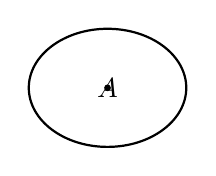
\begin{tikzpicture}[scale=0.5]
\draw[thick] (0,0) ellipse (2 and 1.5);
\filldraw (0,0) circle (2pt);
\node at (0,0) {$A$};
\end{tikzpicture}
\end{center}

\sectiontitle{习题1}

\begin{exercise}
\item 用列举法表示：$\{x\in\mathbb N|x<6\}$；$\{x|x^2-5x+6=0\}$。
\item 用描述法表示：大于$5$的偶数集合。
\item 判断：$\sqrt2\in\mathbb Q$？$0\in\mathbb N$？
\end{exercise}

\newpage

\chaptertitle{第二章\quad 集合的运算与关系}

\sectiontitle{2.1\quad 子集}

\knowbox{
\textbf{子集}：若$A$中每个元素都在$B$中，则$A\subseteq B$。\\
\textbf{真子集}：$A\subseteq B$且$A\neq B$，记作$A\subsetneq B$。\\
\textbf{空集}$\varnothing$：不含任何元素，是任何集合的子集。\\
$n$个元素的集合有$2^n$个子集，$2^n-1$个真子集。}

\begin{center}
\begin{tikzpicture}[scale=0.5]
\draw[thick] (0,0) ellipse (2.5 and 2);
\node at (0,1.6) {$B$};
\draw[thick,fill=lightblue] (-0.3,-0.3) ellipse (1.3 and 1);
\node at (-0.3,1) {$A$};
\end{tikzpicture}
\end{center}

\sectiontitle{2.2\quad 交集与并集}

\knowbox{
交集$A\cap B=\{x|x\in A\text{且}x\in B\}$（公共部分）。\\
并集$A\cup B=\{x|x\in A\text{或}x\in B\}$（全部合起来）。\\
补集$\complement_UA=\{x|x\in U\text{且}x\notin A\}$（在全集中去掉$A$）。}

\begin{center}
\begin{tikzpicture}[scale=0.5]
% 交集
\draw[thick] (-0.8,0) ellipse (1.8 and 1.5);
\draw[thick] (0.8,0) ellipse (1.8 and 1.5);
\begin{scope}
\clip (-0.8,0) ellipse (1.8 and 1.5);
\fill[lightblue] (0.8,0) ellipse (1.8 and 1.5);
\end{scope}
\node at (-1.5,1.2) {$A$};
\node at (1.5,1.2) {$B$};
\node at (0,0) {$A\cap B$};
\end{tikzpicture}
\qquad
\begin{tikzpicture}[scale=0.5]
\draw[thick,fill=lightblue] (-0.8,0) ellipse (1.8 and 1.5);
\draw[thick,fill=lightblue] (0.8,0) ellipse (1.8 and 1.5);
\node at (-1.5,1.2) {$A$};
\node at (1.5,1.2) {$B$};
\end{tikzpicture}
\end{center}

\sectiontitle{习题2}

\begin{exercise}
\item $A=\{1,2,3\}$，写出$A$的所有子集。
\item $A=\{1,2,3,4\}$，$B=\{3,4,5,6\}$，求$A\cap B$、$A\cup B$。
\item 全班$50$人，喜欢数学$30$人，喜欢物理$25$人，两门都喜欢$15$人，求两门都不喜欢的人数。
\item 设$U=\{1,2,3,4,5,6,7\}$，$A=\{2,3,5,7\}$，求$\complement_UA$。
\end{exercise}

\newpage

\chaptertitle{第三章\quad 命题与逻辑}

\sectiontitle{3.1\quad 命题与量词}

\knowbox{
\textbf{命题}：可以判断真假的陈述句。\\
\textbf{全称量词}"任意"（$\forall$）：$\forall x\in A$，$p(x)$成立。\\
\textbf{存在量词}"存在"（$\exists$）：$\exists x\in A$，$p(x)$成立。\\
否定：$\forall$的否定是$\exists$，反之亦然。}

\sectiontitle{3.2\quad 充分条件与必要条件}

\knowbox{
若$p\Rightarrow q$，则$p$是$q$的充分条件，$q$是$p$的必要条件。\\
若$p\Leftrightarrow q$，则$p$是$q$的充要条件。}

\sectiontitle{习题3}

\begin{exercise}
\item 判断真假："如果$x>2$则$x>1$"、"如果两个三角形全等则它们面积相等"。
\item "$x=1$"是"$x^2=1$"的什么条件？
\item 写出"$\forall x\in\mathbb R$，$x^2\ge0$"的否定。
\end{exercise}

\newpage

\chaptertitle{第四章\quad 计数原理}

\sectiontitle{4.1\quad 加法原理与乘法原理}

\knowbox{
\textbf{加法原理}（分类）：总数$=m_1+m_2+\cdots+m_n$（"或"关系）。\\
\textbf{乘法原理}（分步）：总数$=m_1\times m_2\times\cdots\times m_n$（"且"关系）。}

\sectiontitle{4.2\quad 排列}

\knowbox{
从$n$个不同元素中取$m$个按顺序排列：$A_n^m=n(n-1)\cdots(n-m+1)=\dfrac{n!}{(n-m)!}$。\\
$A_n^n=n!$（全排列）。}

\sectiontitle{4.3\quad 组合}

\knowbox{
从$n$个不同元素中取$m$个不计顺序：$C_n^m=\dfrac{A_n^m}{A_m^m}=\dfrac{n!}{m!(n-m)!}$。\\
性质：$C_n^m=C_n^{n-m}$，$C_n^0=1$，$C_n^1=n$。}

\sectiontitle{习题4}

\begin{exercise}
\item 小明有$3$件上衣和$4$条裤子，可以搭配出多少种？
\item 用$1,2,3$能组成多少个无重复数字的三位数？
\item 从$8$人中选$3$人参赛，有多少种选法？
\item $4$人站成一排照相，甲不站两端，有多少种站法？
\item $6$本书选$2$本送人，有几种送法？若选$2$本分别送甲乙两人呢？
\end{exercise}

\newpage

\chaptertitle{第五章\quad 容斥与抽屉原理}

\sectiontitle{5.1\quad 容斥原理}

\knowbox{
两集：$|A\cup B|=|A|+|B|-|A\cap B|$\\
三集：$|A\cup B\cup C|=|A|+|B|+|C|-|A\cap B|-|B\cap C|-|C\cap A|+|A\cap B\cap C|$}

\sectiontitle{5.2\quad 抽屉原理}

\knowbox{
\textbf{第一抽屉原理}：$n+1$个苹果放入$n$个抽屉，必有一个抽屉$\ge2$个苹果。\\
推广：$m$个苹果放入$n$个抽屉（$m>n$），必有至少$\lceil m/n\rceil$个苹果在同一抽屉。}

\sectiontitle{习题5}

\begin{exercise}
\item $1$到$100$中，$2$或$3$的倍数有多少个？
\item $13$人中至少两人同月出生，为什么？
\item 口袋有$3$种颜色的球各$5$个，至少取多少个才能保证有$2$个同色？
\item $1$到$100$中任取$51$个数，必有两个数相差$50$，为什么？
\end{exercise}

\newpage

\chaptertitle{第六章\quad 图论初步}

\sectiontitle{6.1\quad 图的基本概念}

\knowbox{
\textbf{图}：由顶点（点）和边（线）组成。\\
\textbf{度数}：一个顶点连接的边数。\\
\textbf{奇点}：度数为奇数的顶点；\textbf{偶点}：度数为偶数的顶点。\\
\textbf{连通图}：任意两点之间都有路径相连。\\
\textbf{树}：没有圈的连通图，$n$个顶点的树有$n-1$条边。\\
\textbf{完全图}$K_n$：每对顶点之间都有边相连。}

\begin{center}
\begin{tikzpicture}[scale=0.6]
% 树
\begin{scope}
\node at (0,2) {树（6顶点5边）};
\node[circle,draw,fill=lightblue] (a) at (0,0) {$A$};
\node[circle,draw,fill=lightblue] (b) at (-1.5,-1.2) {$B$};
\node[circle,draw,fill=lightblue] (c) at (1.5,-1.2) {$C$};
\node[circle,draw,fill=lightblue] (d) at (-2.5,-2.4) {$D$};
\node[circle,draw,fill=lightblue] (e) at (-0.5,-2.4) {$E$};
\node[circle,draw,fill=lightblue] (f) at (2.5,-2.4) {$F$};
\draw[thick] (a) -- (b) -- (d);
\draw[thick] (b) -- (e);
\draw[thick] (a) -- (c) -- (f);
\end{scope}
% 完全图 K4
\begin{scope}[xshift=6cm]
\node at (0,2) {$K_4$（完全图）};
\node[circle,draw,fill=lightblue] (a) at (-1,0.5) {$A$};
\node[circle,draw,fill=lightblue] (b) at (1,0.5) {$B$};
\node[circle,draw,fill=lightblue] (c) at (-1,-1.5) {$C$};
\node[circle,draw,fill=lightblue] (d) at (1,-1.5) {$D$};
\draw[thick] (a) -- (b) -- (d) -- (c) -- (a);
\draw[thick] (a) -- (d);
\draw[thick] (b) -- (c);
\end{scope}
\end{tikzpicture}
\end{center}

\sectiontitle{6.2\quad 一笔画问题（欧拉路径）}

\knowbox{
\textbf{欧拉定理}：一个连通图可以一笔画成当且仅当奇点个数为$0$或$2$。\\
$0$个奇点：可从任意点出发回到该点（欧拉回路）。\\
$2$个奇点：从一奇点出发结束于另一奇点（欧拉路径）。\\
奇点超过$2$则不能一笔画。\\
应用：七桥问题、路线设计、邮路问题。}

\begin{center}
\begin{tikzpicture}[scale=0.6]
% 可一笔画（2奇点）
\begin{scope}
\node at (0,2.5) {可一笔画（2个奇点）};
\foreach \x/\y/\name in {0/0/A,2/0/B,1/1.5/C} {
  \filldraw (\x,\y) circle (2pt) node[below] {$\name$};
}
\draw[thick] (0,0) -- (2,0) -- (1,1.5) -- (0,0);
\draw[thick] (2,0) -- (1,-0.8) -- (0,0);
\filldraw (1,-0.8) circle (2pt) node[below] {$D$};
\node[red] at (0,-0.3) {$\bullet$};
\node[red] at (2,-0.3) {$\bullet$};
\node at (0,-1.8) {奇点$A,B$};
\end{scope}
% 不能一笔画（4奇点）
\begin{scope}[xshift=5cm]
\node at (0,2.5) {不能一笔画（4奇点）};
\foreach \x/\y/\name in {0/0/A,2/0/B,2/1.5/C,0/1.5/D} {
  \filldraw (\x,\y) circle (2pt) node[below] {$\name$};
}
\draw[thick] (0,0) -- (2,0) -- (2,1.5) -- (0,1.5) -- (0,0);
\draw[thick] (0,0) -- (2,1.5);
\draw[thick] (2,0) -- (0,1.5);
\node[red] at (0,-0.3) {$\bullet$};
\node[red] at (2,-0.3) {$\bullet$};
\node[red] at (2,1.8) {$\bullet$};
\node[red] at (0,1.8) {$\bullet$};
\node at (0,-1.8) {四个奇点};
\end{scope}
\end{tikzpicture}
\end{center}

\sectiontitle{6.3\quad 树与最小生成树}

\knowbox{
\textbf{树}：连通且无圈的图。任意两个顶点之间只有一条路径。\\
\textbf{生成树}：包含原图所有顶点的树。\\
\textbf{最小生成树}：所有边的权值和最小的生成树。\\
应用：铺设道路/线缆使总成本最小（克鲁斯卡尔算法、普里姆算法）。}

\begin{example}
如图，$A$、$B$、$C$、$D$四个城镇之间需要铺设天然气管道，图中标注了各段
距离（单位：千米），求最短的铺设方案。
\end{example}
\begin{solution}
用克鲁斯卡尔算法：每次选权值最小的边且不形成回路。\\
选$AB=3$、$BC=4$、$BD=5$（跳过$AC=6$、$AD=7$、$CD=8$因为会成回路）。\\
最短总长$=3+4+5=12$千米。
\end{solution}

\sectiontitle{习题6}

\begin{exercise}
\item 一个连通图有$4$个奇点，至少需要几笔才能画完？
\item 判断：$3\times3$网格能否一笔画成？
\item 下图是$5$个城市及可建道路的成本（描述），求最小生成树使所有城市连通。
\item 一个连通图有$8$个顶点、$9$条边，它可能是树吗？为什么？
\item 在一笔画问题中，为什么奇点个数为$0$时可以回到起点？
\end{exercise}

\newpage
\sectiontitle{参考答案}

\textbf{习题1}
\begin{enumerate}
\item $\{0,1,2,3,4,5\}$；$\{2,3\}$
\item $\{x\mid x>5,\ x\text{是偶数}\}$（答案不唯一）
\item $\sqrt2\in\mathbb Q$：假；$0\in\mathbb N$：真
\end{enumerate}

\textbf{习题2}
\begin{enumerate}
\item $\varnothing,\{1\},\{2\},\{3\},\{1,2\},\{1,3\},\{2,3\},\{1,2,3\}$
\item $A\cap B=\{3,4\}$，$A\cup B=\{1,2,3,4,5,6\}$
\item $10$人
\item $\{1,4,6\}$
\end{enumerate}

\textbf{习题3}
\begin{enumerate}
\item 真；真
\item 充分不必要条件
\item $\exists x\in\mathbb R$，$x^2<0$
\end{enumerate}

\textbf{习题4}
\begin{enumerate}
\item $12$种
\item $6$个
\item $56$种
\item $12$种
\item 选$2$本送人：$15$种；选$2$本分别送甲乙：$30$种
\end{enumerate}

\textbf{习题5}
\begin{enumerate}
\item $67$个
\item $13$人放入$12$个月，由抽屉原理至少$2$人同月
\item $4$个
\item 将数配对$(1,51),(2,52),\dots,(50,100)$，取$51$个数必有一对同组，差为$50$
\end{enumerate}

\textbf{习题6}
\begin{enumerate}
\item $2$笔
\item 不能（有$8$个奇点）
\item 需根据图的具体数据计算最小生成树
\item 不是树（树有$n-1=7$条边，该图有$9$条边）
\item 奇点数为$0$时存在欧拉回路，可一笔画成并回到起点
\end{enumerate}

\end{document}
